% Poenostavljena ponazoritev rojenja delcev (RD) za sliko fig:pso-illus.
% Prevedi:  pdflatex optimizer_pso_illus.tex   (v mapi thesis-paper/fig)
% Delovanje sledi Curi (2009) in portfolio_optimizers/pso.cpp:
%   v^{t+1} = v^t + w1 (x^G - x) + w2 (x* - x),  x^{t+1} = x + v^{t+1},  w1, w2 ~ U[0,2];
%   osebno najboljša rešitev x* se posodobi le ob izboljšanju,
%   najboljša rešitev roja x^G je najboljša med osebno najboljšimi.
\RequirePackage{fix-cm} % zvezno skaliranje pisave CM (sicer se manjše velikosti zaokrožijo na 5 pt)
\documentclass[tikz,border=2pt]{standalone}
\usepackage[utf8]{inputenc}
\usepackage[T1]{fontenc}
\usetikzlibrary{arrows.meta,shapes.geometric,calc}
\renewcommand{\vec}[1]{\ensuremath{\mathbf{#1}}}

\definecolor{part}{HTML}{1A63C6}
\definecolor{pbest}{HTML}{A983D8}
\definecolor{gbest}{HTML}{C00000}
\definecolor{move}{HTML}{D2691E}
\definecolor{pcomp}{HTML}{6A1B9A}
\definecolor{inert}{HTML}{6B6B6B}
\definecolor{iso}{HTML}{2F6FA8}

\tikzset{
  particle/.style={circle,fill=part,draw=white,line width=0.4pt,inner sep=0pt,minimum size=9pt,
                   font=\fontsize{4}{4.5}\selectfont\bfseries,text=white},
  ghost/.style={circle,draw=part!50,fill=white,line width=0.6pt,inner sep=0pt,minimum size=9pt,
                font=\fontsize{4}{4.5}\selectfont\bfseries,text=part!55},
  newpos/.style={circle,draw=move,densely dashed,fill=white,line width=0.8pt,inner sep=0pt,minimum size=9pt,
                 font=\fontsize{4}{4.5}\selectfont\bfseries,text=move},
  lab/.style={font=\fontsize{6}{7}\selectfont,inner sep=1pt},
  pb/.style={diamond,fill=pbest,inner sep=0pt,minimum size=12pt},
  gb/.style={diamond,fill=pbest,draw=gbest,line width=1.1pt,inner sep=0pt,minimum size=12pt},
  vec/.style={-{Stealth[length=4pt,width=3.4pt]},line width=1pt},
  ttl/.style={font=\small},
}

% okvir in izolinije ciljne funkcije g(w) (minimum v w*)
\newcommand{\panel}[1]{%
  \begin{scope}
    \clip (0,0) rectangle (4,5);
    \fill[iso!6] (0,0) rectangle (4,5);
    \foreach \rx/\ry/\o in {3.4/2.1/10, 2.6/1.6/16, 1.9/1.15/24, 1.25/0.75/34, 0.6/0.38/46}
      \filldraw[fill=iso,fill opacity=0.09,draw=iso!55,densely dashed,line width=0.35pt]
        (2.6,2.8) [rotate around={-35:(2.6,2.8)}] ellipse ({\rx} and {\ry});
  \end{scope}
  \draw[line width=0.5pt,black!70] (0,0) rectangle (4,5);
  \node[ttl,above] at (2,5) {#1};
  \node[star,star points=5,star point ratio=2.3,fill=gbest,draw=white,line width=0.4pt,
        inner sep=0pt,minimum size=11pt] at (2.6,2.8) {};
}

\begin{document}
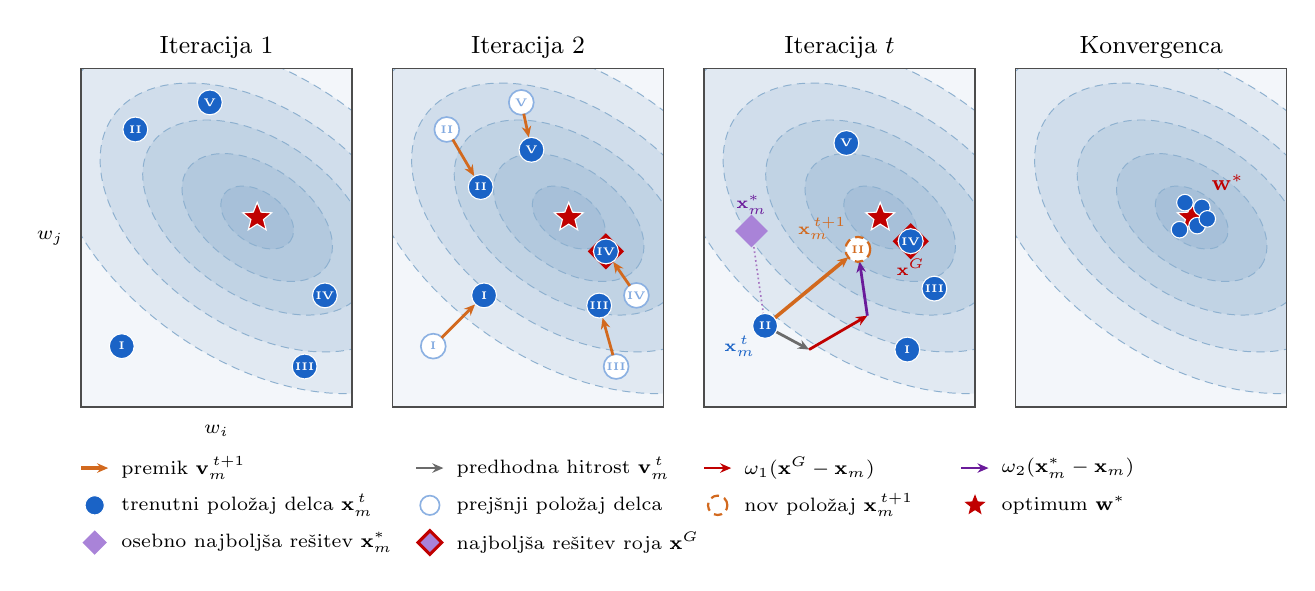
\begin{tikzpicture}[x=0.86cm,y=0.86cm]

% ---------------- Iteracija 1: naključni začetni položaji; osebni optimum = začetni položaj (ne rišemo posebej)
\begin{scope}
  \panel{Iteracija $1$}
  \foreach \p/\x/\y in {I/0.6/0.9, II/0.8/4.1, III/3.3/0.6, IV/3.6/1.65, V/1.9/4.5}
    { \node[particle] at (\x,\y) {\p}; }
  \node[font=\scriptsize,anchor=north] at (2,-0.12) {$w_i$};
  \node[font=\scriptsize,anchor=east] at (-0.12,2.5) {$w_j$};
\end{scope}

% ---------------- Iteracija 2: vsi delci se izboljšajo, osebni optimum = nov položaj (ne rišemo posebej)
\begin{scope}[shift={(4.6,0)}]
  \panel{Iteracija $2$}
  \foreach \p/\ax/\ay/\bx/\by in {I/0.6/0.9/1.35/1.65, II/0.8/4.1/1.3/3.25, III/3.3/0.6/3.05/1.5,
                                  IV/3.6/1.65/3.15/2.3, V/1.9/4.5/2.05/3.8}
    { \node[ghost] at (\ax,\ay) {\p};
      \draw[vec,move,shorten <=4.2pt,shorten >=4.6pt] (\ax,\ay) -- (\bx,\by);
      \node[particle] at (\bx,\by) {\p}; }
  \node[gb] at (3.15,2.3) {}; \node[particle] at (3.15,2.3) {IV};
\end{scope}

% ---------------- Iteracija t: delec II se je poslabšal; osebni optimum x* je eden od prejšnjih položajev
% Komponente so narisane zaporedno (vztrajnost -> omega1 -> omega2), da je pot konveksna in
% rezultanta (premik) ne seka nobene komponente. Geometrija preverjena: g(x*) < g(x), g(x^G) najmanjši.
\begin{scope}[shift={(9.2,0)}]
  \panel{Iteracija $t$}
  \foreach \p/\x/\y in {I/3.0/0.85, III/3.4/1.75, V/2.1/3.9}
    { \node[particle] at (\x,\y) {\p}; }
  % najboljša rešitev roja x^G = osebni optimum delca IV
  \coordinate (xg) at (3.05,2.45);
  \node[gb] at (xg) {}; \node[particle] at (xg) {IV};
  % delec II: položaj x in osebni optimum x*
  \coordinate (x)  at (0.9,1.2);
  \coordinate (xs) at (0.7,2.6);
  \node[pb] at (xs) {};
  \draw[pcomp!60,densely dotted,line width=0.6pt,shorten <=4.2pt,shorten >=5pt] (x) -- (xs);
  % v^t = (0.65,-0.35);  w1 (x^G-x) = 0.4 (2.15,1.25);  w2 (x*-x) = 0.7 (-0.2,1.4)
  \coordinate (a) at ($(x)+(0.65,-0.35)$);
  \coordinate (b) at ($(a)+(0.86,0.5)$);
  \coordinate (c) at ($(b)+(-0.14,0.98)$);
  \draw[vec,inert,shorten <=4.2pt] (x) -- (a);
  \draw[vec,gbest] (a) -- (b);
  \draw[vec,pcomp,shorten >=4.4pt] (b) -- (c);
  \draw[vec,move,line width=1.3pt,shorten <=4.2pt,shorten >=4.4pt] (x) -- (c);
  \node[newpos] at (c) {II};
  \node[particle] at (x) {II};
  \node[lab,anchor=north east,part] at ($(x)+(-0.1,-0.1)$) {$\vec{x}^{\,t}_{m}$};
  \node[lab,anchor=south east,move] at ($(c)+(-0.12,0.1)$) {$\vec{x}^{\,t+1}_{m}$};
  \node[lab,anchor=south,pcomp] at ($(xs)+(0,0.2)$) {$\vec{x}^{\ast}_{m}$};
  \node[lab,anchor=north,gbest] at ($(xg)+(0,-0.22)$) {$\vec{x}^{G}$};
\end{scope}

% ---------------- Konvergenca
\begin{scope}[shift={(13.8,0)}]
  \panel{Konvergenca}
  \foreach \p/\x/\y in {I/2.42/2.62, II/2.75/2.95, III/2.5/3.02, IV/2.68/2.68, V/2.83/2.78}
    { \node[particle,minimum size=6pt,font=\fontsize{1}{1}\selectfont,text=part] at (\x,\y) {}; }
  \node[font=\footnotesize,gbest,anchor=south west] at (2.75,3.05) {$\vec{w}^{\ast}$};
\end{scope}

% ---------------- Legenda (vrstice: vektorji, položaji, najboljše rešitve; stolpci poravnani)
\begin{scope}[shift={(0,-0.9)},font=\scriptsize]
  \draw[vec,move,line width=1.2pt] (0,0) -- (0.4,0);
  \node[anchor=west] at (0.45,0) {premik $\vec{v}^{\,t+1}_m$};
  \draw[vec,inert] (4.95,0) -- (5.35,0);
  \node[anchor=west] at (5.4,0) {predhodna hitrost $\vec{v}^{\,t}_m$};
  \draw[vec,gbest] (9.2,0) -- (9.6,0);
  \node[anchor=west] at (9.65,0) {$\omega_1(\vec{x}^{G}-\vec{x}_m)$};
  \draw[vec,pcomp] (13.0,0) -- (13.4,0);
  \node[anchor=west] at (13.45,0) {$\omega_2(\vec{x}^{\ast}_m-\vec{x}_m)$};

  \node[particle,minimum size=7pt] at (0.2,-0.55) {};
  \node[anchor=west] at (0.45,-0.55) {trenutni položaj delca $\vec{x}^{\,t}_m$};
  \node[ghost,minimum size=7pt] at (5.15,-0.55) {};
  \node[anchor=west] at (5.4,-0.55) {prejšnji položaj delca};
  \node[newpos,minimum size=7pt] at (9.4,-0.55) {};
  \node[anchor=west] at (9.65,-0.55) {nov položaj $\vec{x}^{\,t+1}_m$};
  \node[star,star points=5,star point ratio=2.3,fill=gbest,inner sep=0pt,minimum size=8pt] at (13.2,-0.55) {};
  \node[anchor=west] at (13.45,-0.55) {optimum $\vec{w}^{\ast}$};

  \node[pb,minimum size=9pt] at (0.2,-1.1) {};
  \node[anchor=west] at (0.45,-1.1) {osebno najboljša rešitev $\vec{x}^{\ast}_m$};
  \node[gb,minimum size=9pt] at (5.15,-1.1) {};
  \node[anchor=west] at (5.4,-1.1) {najboljša rešitev roja $\vec{x}^{G}$};

\end{scope}
\end{tikzpicture}
\end{document}
